\documentclass[]{IEEEphot}

\usepackage{setspace}
\usepackage{tikz}
\usepackage{amsmath, amssymb}
\usepackage{slashbox}
\usepackage{algorithm,algpseudocode}
\usepackage{mathrsfs}

\classnumber{CS 5300}

\newtheorem{theorem}{Theorem}
\newtheorem{lemma}{Lemma}

\begin{document}
	
	\title{An Analysis\\ of \\ Branch-and-Bound}
	
	\author{~Rick Ramirez \\ Ruben Bramasco}
	
	\affil{California State Polytechnic University, Pomona}
	\maketitle
	\markboth{Fall 2021}{Advanced Algorithm Design and Analysis}
	\vspace{-2cm}
	\begin{center}
    	
\includegraphics[width=5cm]{images/primary-logo-inside-stacked}\\
    \end{center}
	\vspace{0.25cm}

	\begin{abstract}
		\doublespacing\small
		The Branch-and-Bound paradigm is a widely used framework for solving combinatorial optimization problems.
		Here we describe the general algorithm and analyze it's time complexity.
		We follow this with a discussion of recent improvements of the branch-and-bound framework in the wake of quantum computation and describe how a quantum algorithm could produce a quadratic acceleration of the classical time complexity.
	\end{abstract}

	\begin{IEEEkeywords}
		Branch-and-Bound, Pruning rules, Branching strategy, Ising model, Quantum walk
	\end{IEEEkeywords}

	%! Author = rickr
%! Date = 11/17/2021

\section{Introduction}
	The branch-and-bound design paradigm has proven exceedingly useful in solving combinatorial optimization problems with applications in artificial intelligence, applied mathematics and theoretical computer science. 
	The design can be applied to any problem where the goal is to find a minimum-cost solution in a setting where one has access to a bounding function that returns a lower bound on a given subset of solutions and a branching rule that can be applied to partition a subset if possible solutions cannot be ruled out. 
	The technique has been used in solving a number of NP-hard problems and may also serve as the base of various heuristics.\\
	\indent
	The success of branch-and-bound has also sparked interest in applications involving quantum computation by encoding optimization problems to the ground state of classical spin systems. 
	This has led to the development of quantum branch-and-bound algorithms and have been shown to increase performance significantly. 
	
	
	
	
	%! Author = rickr
%! Date = 11/17/2021

\section{Basic Idea Behind BnB}
	
	%! Author = rickr
%! Date = 11/17/2021

\section{Integer Constraint Problems}
	
	%! Author = rickr
%! Date = 11/17/2021

\section{TSP Better Lower Bound}
    There are problems like the traveling salesman problem in this example
    that are easy to model using branch-and-bound but do not see too much improvements.
    The reason BnB does not work well with TSP is because BnB relies on pseudo
    parallelism. BnB will choose to expand best possible path each time, and 
    with a problem like TSP, the best possible path will almost always be the 
    last expanded path. This makes the algorithm almost useless since you 
    would expand almost every combination of tour, and essentially brute-force the solution.
    To combat this researchers have used heuristics, in hopes of making a better
    choice for a lower-bound.

    \subsubsection{Creating a Better Lower Bound}
    Firstly, our lower-bound calculation before our heuristic is simply the sum 
    of the tour edges. To improve this we will utilize an encoding scheme known as 
    a graph adjacency matrix, and reduce it. There are two reasons for the reduction, 
    the first is that reduction keeps track of our current state of the tour, and the second
    is that the cost of reduction is an admissible heuristic in the TSP problem.
    The idea is that the cost of reduction is equal to the shortest possible edges left to
    take on the graph. Note, the shortest edges do not have to be constrained to the tour, they
    are just simply the shortest edges coming out of each node. To compute the reduction, take the
    shortest number in each row, then subtract it from each element, finally sum the shortest edges.
    The outputted matrix becomes the new state of the child branch and used to compute it's lower-bound.\\

    After computing the reduction cost we can now make our lower bound calculation.
    \begin{equation}
        LB = LB_p + w(p, n) + R(M_n)
    \end{equation}
    Where $LB_p$ is the lower-bound of the parent, $w(p, n)$ is the weight of the edge
    between the parent, and $R(M_n)$ is the cost of reduction. 
    
    It is important to realize that branch-and-bound is not one size fits all algorithm, so
    although there maybe a problem that can be encoded with an adjacency matrix, it does not mean
    there exist an admissible heuristic for it. 

   \begin{equation}
	    \begin{vmatrix}
	        \infty & 9 & 2 & 8\\
	        9 & \infty & 7 & 3 \\
	        2 & 7 & \infty & 4 \\
	        8 & 3 & 4 & \infty
	    \end{vmatrix}
	        %!c = 2 + 3 + 2 + 3
	    \begin{vmatrix}
	        \infty & 7 & 0 & 6\\
	        6 & \infty & 4 & 0 \\
	        0 & 5 & \infty & 2 \\
	        5 & 0 & 1 & \infty
	    \end{vmatrix}
	\end{equation}

	
	%! Author = rickr
%! Date = 11/17/2021

\section{When Is BnB Viable}
	
	%! Author = rickr
%! Date = 11/17/2021

\section{Advancing Branch And Bound}

	
	%! Author = rickr
%! Date = 11/17/2021
\newpage
\section{Traveling Salesman Problem To Ising Model}
	Recent interest in solving NP-complete and NP-hard problems via adiabatic quantum optimization has led to convenient transformations of Ising formulations. The idea is that if one problem has a quantum Hamiltonian $H_p$ whose ground state energy encodes the solution to a problem of interest, and another Hamiltonian $H_0$, whose ground state is "easy" to find and prepare, then we can prepare the system to be in the ground state of $H_0$ before adiabatically changing it in terms of $H_p$ for a time $T$ \cite{lucas2014ising}. So long as $T$ is large enough and $H_0$ and $H_p$ do not commute, the system should remain in the resulting ground state for all time. Therefore, measuring the ground state of the system at time $T$ will return a solution to the problem of interest. Though there has been debate on the practicality of such a method, there has been extensive effort in finding formulations of various NPC and NPH problems in terms of Ising models. Here we present one such transformation and show how it can be used to improve the computation time of a generic Branch-and-Bound technique. 
	\subsection{TSP to Hamiltonian Circuit}
		Consider an instance of the Traveling Salesman problem for the graph $G = (V,E)$ as shown in Figure \ref{fig:tsp}.
		Each edge $uv$ has a weight $W_{uv}$ associated with it. 
		\begin{figure}[h]
			\begin{center}
				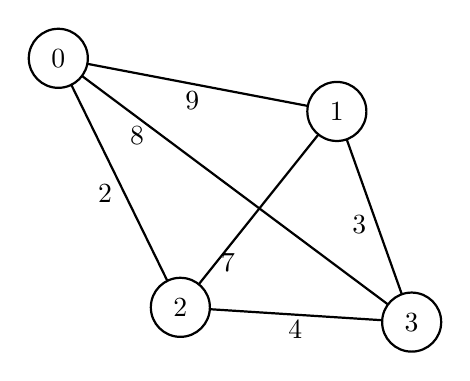
\begin{tikzpicture}[scale=0.125]
					\tikzstyle{every node}+=[inner sep=0pt]
					\draw  [thick](22,-14.2) circle (3);
					\draw  [][thick](22,-14.2) node {$0$};
					\draw  [thick](34.4,-39.5) circle (3);
					\draw  [][thick](34.4,-39.5) node {$2$};
					\draw  [thick](50.3,-19.6) circle (3);
					\draw  [][thick](50.3,-19.6) node {$1$};
					\draw  [thick](57.9,-41) circle (3);
					\draw  [][thick](57.9,-41) node {$3$};
					\draw  [][thick](23.32,-16.89) -- (33.08,-36.81);
					
					\draw [](27.5,-27.94) node [left] {$2$};
					\draw [][thick] (24.95,-14.76) -- (47.35,-19.04);
					
					\draw [](35.62,-17.49) node [below] {$9$};
					\draw [][thick] (51.3,-22.43) -- (56.9,-38.17);
					
					\draw [](53.34,-31.06) node [left] {$3$};
					\draw [][thick] (37.39,-39.69) -- (54.91,-40.81);
					
					\draw [](46.07,-40.81) node [below] {$4$};
					\draw [][thick] (24.4,-15.99) -- (55.5,-39.21);
					
					\draw [](30,-23) node [above] {$8$};
					\draw [][thick] (48.43,-21.94) -- (36.27,-37.16);
					
					\draw [](40, -35) node [left] {$7$};
				\end{tikzpicture}\caption{A graph G representing an instance of the Traveling Salesman Problem. Each node $V$ is connected via a weighted edge $E=W_{uv}$. }\label{fig:tsp}
			\end{center}
		\end{figure}\\
		The set of solutions to this graph can be seen in Table \ref{tab:eigenset} located in the appendix and the shortest Hamiltonian cycle that can be taken has a total distance of 18.
		One possible route is $2\rightarrow3\rightarrow1\rightarrow0$. 
		This route can be represented as a matrix as shown if Figure \ref{fig:matrix}, where $i$ and $p$ correspond to the city and order of traversal respectively. 
		\begin{figure}[h]
			\begin{center}
					\begin{tabular}{c|cccc}
					\backslashbox{i}{p}&0 &1 &2 &3 \\
					\hline
					0& 0&0&0&1\\
					
					1& 0&0&1&0\\
					
					2& 1&0&0&0\\
					
					3& 0&1&0&0\\
				\end{tabular}
			\end{center}\caption{Solution to TSP in Figure \ref{fig:tsp} represented in the form of a matrix. The column $i$ represents each node, and the row $p$ corresponds to the nodes position in the traversal. A decision variable value of 1 corresponds to the path being taken.}\label{fig:matrix}
		\end{figure}\\
		The solution matrix of Figure \ref{fig:matrix} can be unpacked into the form of a vector 
		\begin{equation}
			\vec{x} = \langle x_1, x_2, \dots, x_{N^2} \rangle
			\label{eq:vector}
		\end{equation}
		such that $x_j = x_{N \cdot i+p}$ where $N$ is the number of nodes in the graph. 
		For example, the value at $x_{2,1}$ in the matrix will map to $x_9$ in the vector. Therefore, the vector representation of the solution to TSP in Figure \ref{fig:tsp} is $\vec{x} = <0,0,0,1,0,0,1,0,1,0,0,0,0,1,0,0>$. 
		Applying the cost function to the eigenvector will result in an eigenvalue of $C(\vec{x}) = 18$.\\
		
		For nodes forming a traversal such that $x_{i,p}$ and $x_{i,p+1}$ are both equal to one but not connected in $G$, i.e., $(i,j)\notin E$, then an energy penalty should be imposed in the form $\sum_{i,j \notin E}\sum_p x_{i,p}x_{i,p+1}>0$ \cite{lucas2014ising}.
		However, since we are only considering fully connected graphs, this term may be omitted and the net cost of a tour can be calculated from the cost function of Equation \ref{eq:cost}.
		% Cost Function
		\begin{equation}
			C(X)=\sum_{i,j}w_{i,j} \sum_p x_{i,p}x_{j,p+1} 
			\label{eq:cost}
		\end{equation}
		Inspecting the features of Figure \ref{fig:matrix}, we find that every vertex can only appear once in a cycle and each position must be occupied by a node. 
		This amounts to the two constraints given in Equation \ref{eq:constraints}.
		% Constraints
		\begin{equation}
			\sum_p x_{i,p}=1 \quad \forall \: i \in cities \quad \text{and} \quad \sum_i x_{i,p}=1 \quad \forall \: p \in route
			\label{eq:constraints}
		\end{equation}
		By imposing these constraints to Equation \ref{eq:cost}, we find that the objective function to be minimized takes the form
		% Distance with constraints
		\begin{equation}
			C(X)=\sum_{i,j}w_{i,j} \sum_p x_{i,p}x_{j,p+1} + A\sum_p (1 - \sum_i x_{i,p})^2 + A\sum_i (1 - \sum_p x_{i,p})^2
			\label{eq:hamiltoniancircuit}
		\end{equation}
		where $A>W_{max}$ is a positive constant set to be much larger than maximum weight encountered during the traversal. Note that the constraints are squared so as to prevent the algorithm from diverging to negative infinity. \\
	
		To complete the preparation of TSP, we need to convert the cost function of Equation \ref{eq:cost} into a quantum Hamiltonian by changing variables from $x_i$ to the Pauli operator $\sigma_i^z$ (a $2x2$ matrix whose eigenvectors $|1,0\rangle$ and $|0,-1\rangle$ have eigenvalues (+1,-1)). 
		\begin{equation}
			x_i \rightarrow \frac{ 1-\sigma_{i,p}^z}{2} \qquad \Rightarrow \qquad C(X) \rightarrow C(\sigma_{i,p}^z) \equiv H_p
			\label{eq:transformation}
		\end{equation}
	
	\subsection{The Ising Model}
		In ideal \textit{paramagnetism} (magnetism where materials are weakly attracted by an external magnetic field) microscopic magnetic dipole moments respond only to an external field. 
		However, in the real world, neighboring atomic dipoles are influenced by each other. 
		When neighboring dipoles align parallel, even in the absence of an external field, we call the material a ferromagnet. 
		The Ising model is a mathematical model used to describe ferromagnetism in terms of statistical mechanics. The model consists of discrete variables that represent the magnetic dipole moments of atomic spins and can have a value of $\pm 1$. 
		The variables are used to describe preference for neighboring dipoles to align parallel or anti-parallel to each other \cite{schroeder2011thermal}.
		
		\begin{figure}[h]
			\begin{center}
				\includegraphics[width=4cm]{images/lattice}
			\end{center}
			\caption{Atomic spin states arranged into a 2-dimensional lattice structure under periodic boundary conditions. The energy of the particle at lattice site $k$ has a value $E = -2J$ and the total energy of the system is found by summing over the entire structure.}\label{fig:lattice}
		\end{figure}
	
		For example, consider a lattice of particles as shown in Figure \ref{fig:lattice}. 
		Each particle has an associated spin state that can take the orientations of spin-up $|+\rangle$ or spin-down $|-\rangle$ with values $\sigma_k = +1$ and $\sigma_k = -1$ respectively. The energy associated with the particle at lattice site $k$ is found to be 
		\begin{equation}
			 E_k= - J\sum_{<i,j>}\sigma_k^i\sigma_k^j \quad \cite{ising1925beitrag}
			\label{eq:latticeSiteEnergy}
		\end{equation}
		where $J$ is a coupling constant, $\sigma_k$ is a discrete variable, and $<i,j>$ means to sum over the nearest neighbors. Note that for parallel spins, $J>0$, for anti-parallel spins $J<0$, and for no interaction $J = 0$. 
		In the presence of a magnetic field $\vec{B}$, the kinetic and potential energy of the system can be represented by the Hamiltonian
		\begin{equation}
			H = \frac{g_s}{2}\mu_B B\sum_{i=1}^N \sigma_z^i - J\sum_{<i,j>}\sigma_z^i\sigma_z^j
			\label{eq:isingHamiltonian}
		\end{equation} 
		where the spin g-factor for an electron $g_s$ and the Bohr magneton $\mu_B$ are constants, and the discrete variable $\sigma_k$ has been replaced with the Pauli z-operator $\sigma_z$ as in Equation \ref{eq:transformation}. 
		There are many techniques for solving generalized Ising models including transfer matrix methods\cite{onsager1944crystal}, graphical/combinatorial methods\cite{feynman1972statistical}, and Monte Carlo simulations\cite{schroeder2011thermal}. 
		However, with the advent of quantum computation, the time independent Schrodinger equation is especially convenient.  
	\subsection{Time Independent Schrodinger Equation}
		In quantum mechanics, the Schrodinger equation is a partial differential equation that governs the dynamics of the wave function $\Psi(x,t)$ of a particle in a system. 
		In essence, it is an accounting of energy where the kinetic and potential energy are encapsulated in a single operator called a Hamiltonian, and the total energy of the system is set to be the time derivative acting on the wave function. 
		Since the Ising model focuses on the spin configuration of a particle and neglects the space and time components, we can utilize a time independent version of the Schrodinger equation and treat it as an eigenvalue problem as shown in Equation \ref{eq:tise}. 
		
		\begin{equation}
			H | \Psi \rangle = E | \Psi \rangle
			\label{eq:tise}
		\end{equation}
	
		As the Hamiltonian operator acts on the wave function, a scalar value is produced along with the same vector. 
		In terms of linear algebra, the wave function $| \Psi \rangle$ can be treated as an eigenvector with a corresponding eigenvalue $E$. 
		Note that each eigenvalue can correspond to a set of eigenvectors and that minimizing Equation \ref{eq:tise} is to solve for the ground state energy of the system. \\
		
		Relating this back to the Traveling Salesman problem, recall that in Equation \ref{eq:transformation} we transformed the cost function into the same form as the Ising Hamiltonial of Equation \ref{eq:isingHamiltonian}. We now need to map the solution vector of Equation \ref{eq:vector} into qubits to be fed into a quantum computer. 
		\begin{equation}
			\vec{x} = \langle x_1, x_2, \dots, x_{N^2} \rangle \rightarrow |\Psi\rangle = |x_1\rangle \otimes |x_2\rangle \dots \otimes  |x_{N^2}\rangle 
		\end{equation}
		Note we do not require a transformation between the energy of the Schrodinger equation and the distance of the Hamiltonian Circuit because both quantities are scalars. This completes the transformation from the Traveling Salesman problem into the Ising model. The solution for the ground state energy of the Ising Hamiltonian corresponds directly to the minimum tour distance in TSP however in this form, we are able to exploit the features of quantum mechanics and obtain a solution in less time. 

	
	%! Author = rickr
%! Date = 11/17/2021
\newpage
\section{Quantum Improvements}
	With the recent advancements in quantum computing, access to hardware has become readily available to the general public and quantum algorithms have been shown to perform exponentially better than some of their classical counterparts for select problems. 
	For example, Grover's algorithm can sort through and find an element within an unstructured set using $O(\sqrt{N})$ operations as oppose to the $O(N)$ performance of an exhaustive search. However, for many problems, it's is more beneficial to utilize techniques found in classical algorithms that take advantage of the structure of a problem. One such technique is Branch-and-bound. 
	By applying the Branch-and-Bound paradigm in a quantum setting, it is possible to achieve a near quadratic improvement beyond that of classical pruning techniques \cite{montanaro2020quantum}. \\
	

	Though there are several different implementations of quantum computing systems, the most popular is the quantum circuit.
	The model is based on the concept of a qubit which is analogous to the bit in classical computing. 
	The qubit acts as the basic unit of quantum information and is physically realized as the spin state of a fermion (a particle with a half integer spin; typically 1/2). 
	Since the qubit is measured as the spin state of a particle, it's properties are governed by the wave function of that particle $|\Psi\rangle$. 
	For example, since the quantum spin number of a qubit is 1/2, it can exist in one of two states (spin up $|0\rangle$ or spin down $|1\rangle$) when measured. 
	However, before the measurement, the particle can be in a superposition of both states 
	\begin{equation}
		|\Psi\rangle = \alpha |0\rangle + \beta|1\rangle
		\label{eq:spinStates}
	\end{equation}
	where $\alpha$ and $\beta$ are probability amplitudes such that $|\alpha|^2+|\beta|^2 = 1$.
	This means that unlike a classical bit that can discretely take on a value of $0$ \textit{or} $1$, the qubit can exist in a state of $0$ \textit{and} $1$ simultaneously. We can exploit this feature of quantum mechanics to increase the speed of classical algorithms by placing the qubit into a superposition of states and letting the system evolve in time before taking a measurement. 
	
	\subsection{Classical vs Quantum Walk}
	
		Consider the case of a classical random walk. In this example we search for a marked node within a binary tree of size $n$ nodes. 
		If we have no indication of where in the tree the target might be, then a sure proof way of finding it is to visit each node, one step at a time, with $50\%$ probability of taking a step to the left and $50\%$ probability of taking a step to the right. 
		Naturally, for every step away from the origin, there is an equal probability of taking a step back toward the origin, and over time we will obtain a normal Gaussian distribution of steps as shown in Figure \ref{fig:quantumWalk}. 
		The classical random walk distribution exhibits a variance of 
		\begin{equation}
			\sigma^2 \propto n
		\end{equation}
		which is to say that there is a very low probability of hitting the target if it is far away from the origin.
		Since  each step is based on a set of definite states, the randomness of the traversal is caused by a stochastic transition between states.
		Now consider a random walk in a quantum setting. 
		In this case, the randomness comes from the quantum superposition imposed by Equation \ref{eq:spinStates}, a reversible unitary evolution (typically in the form of a Hadamard coin), and a collapse of the wave-function when a measurement is actually taken. 
		Another difference between the quantum and classical random walk is the time at which a measurement is taken. 
		In the classical version, it makes no difference to take measurements at each iteration, however in the quantum version, if a measurement of the wave-function is taken at each iteration, then the distribution converges to the classical Gaussian form. 
		If the wave-function is left to interfere with itself before a measurement is taken, then the probability distribution is much more intricate, as can be seen in Figure \ref{fig:quantumWalk}.
		It can be shown the after $n$ steps, the quantum walk obtains a variance of 
		\begin{equation}
			\sigma^2 \propto n^2 \quad\cite{kempe2003quantum}
		\end{equation}
		Therefore, the quantum walk propagates quadratically faster than the classical walk, and this speed increase can be applied to the branch-and-bound framework. 
		From Figure \ref{fig:quantumWalk}, if the wave-function is placed in a superposition, then the distribution exhibits destructive interference about the origin.
		However, if the wave-function begins in a pure spin-up or spin-down configuration, then it is possible to create a bias toward any particular direction as shown in Figure \ref{fig:biasWalk} of the appendix.
	\begin{figure}[h]
		\begin{center}
			\includegraphics[width=12cm]{images/afunc2}
		\end{center}
		\caption{Difference between quantum and classical random walk. The blue dotted line represents the Gaussian distribution created by the classical walk and has a variance $\sigma^2 \propto n$. The black distribution is the result of the quantum random walk where the initial wave-function placed into a superposition $|\Psi\rangle = \alpha|0\rangle + \beta|1\rangle$ and acted on my a balanced Hadamard coin. The quantum distribution exhibits a variance of $\sigma^2 \propto n$ with de-constructive interference about the origin and constructive interference at the edges of propagation.}
		\label{fig:quantumWalk}
	\end{figure}\\
	To summarize the results, consider three individual cases of solving combinatorial problems with Hamiltonians similar to that of Equation \ref{eq:isingHamiltonian}.
	One case is solved using classical branch-and-bound techniques, one is solved using quantum walks, and one is solved using branch-and-bound in a quantum setting. 
	If the classical branch-and-bound techniques are applied to solve for the largest known ground states of the Beransconi model, the runtime is roughly $O(2^{0.79n})$ \cite{packebusch2016low}. 
	If we apply a quantum walk to classical algorithms that solve the Sherrington-Kirkpatrick model (an Ising model with long range anti-ferrmagnetic couplings) then it has been shown we can increase runtime to approximately $O(2^{0.41n})$ \cite{callison2019finding}. 
	Finally, by applying quantum branch-and-bound algorithms to the same model, it has been shown the runtime can be increased further to $O(2^{0.226})$ \cite{montanaro2020quantum}.

	
	\input{sections/Conclusion.tex}
	
	\newpage
	\bibliographystyle{IEEEtran}
	\bibliography{groupPaper}
	
	\newpage
\appendix
\begin{table}[h]
	\[
	\begin{split}
		&0 \rightarrow 1 \rightarrow 2 \rightarrow 3 \rightarrow 0 \quad \text{dist}=28 \hspace{1cm} 1 \rightarrow 0 \rightarrow 2 \rightarrow 3 \rightarrow 1 \quad \text{dist}=18 \\
		&0 \rightarrow 1 \rightarrow 3 \rightarrow 2 \rightarrow 0 \quad \text{dist}=18 \hspace{1cm} 1 \rightarrow 0 \rightarrow 3 \rightarrow 2 \rightarrow 1 \quad \text{dist}=28\\
		&0 \rightarrow 2 \rightarrow 1 \rightarrow 3 \rightarrow 0 \quad \text{dist}=20 \hspace{1cm} 1 \rightarrow 2 \rightarrow 0 \rightarrow 3 \rightarrow 1 \quad \text{dist}=20\\
		&0 \rightarrow 2 \rightarrow 3 \rightarrow 1 \rightarrow 0 \quad \text{dist}=18 \hspace{1cm} 1 \rightarrow 2 \rightarrow 3 \rightarrow 0 \rightarrow 1 \quad \text{dist}=28\\
		&0 \rightarrow 3 \rightarrow 1 \rightarrow 2 \rightarrow 0 \quad \text{dist}=20 \hspace{1cm} 1 \rightarrow 3 \rightarrow 0 \rightarrow 2 \rightarrow 1 \quad \text{dist}=20\\
		&0 \rightarrow 3 \rightarrow 2 \rightarrow 1 \rightarrow 0 \quad \text{dist}=28 \hspace{1cm} 1 \rightarrow 3 \rightarrow 2 \rightarrow 0 \rightarrow 1 \quad \text{dist}=18\\ \\
		%
		&2 \rightarrow 0 \rightarrow 1 \rightarrow 3 \rightarrow 2 \quad \text{dist}=18 \hspace{1cm} 3 \rightarrow 0 \rightarrow 1 \rightarrow 2 \rightarrow 3 \quad \text{dist}=28 \\
		&2 \rightarrow 0 \rightarrow 3 \rightarrow 1 \rightarrow 2 \quad \text{dist}=20 \hspace{1cm} 3 \rightarrow 0 \rightarrow 2 \rightarrow 1 \rightarrow 3 \quad \text{dist}=20\\
		&2 \rightarrow 1 \rightarrow 0 \rightarrow 3 \rightarrow 2 \quad \text{dist}=28 \hspace{1cm} 3 \rightarrow 1 \rightarrow 0 \rightarrow 2 \rightarrow 3 \quad \text{dist}=18\\
		&2 \rightarrow 1 \rightarrow 3 \rightarrow 0 \rightarrow 2 \quad \text{dist}=20 \hspace{1cm} 3 \rightarrow 1 \rightarrow 2 \rightarrow 0 \rightarrow 3 \quad \text{dist}=20\\
		&2 \rightarrow 3 \rightarrow 0 \rightarrow 1 \rightarrow 2 \quad \text{dist}=28 \hspace{1cm} 3 \rightarrow 2 \rightarrow 0 \rightarrow 1 \rightarrow 3 \quad \text{dist}=18\\
		&2 \rightarrow 3 \rightarrow 1 \rightarrow 0 \rightarrow 2 \quad \text{dist}=18 \hspace{1cm} 3 \rightarrow 2 \rightarrow 1 \rightarrow 0 \rightarrow 3 \quad \text{dist}=28\\
	\end{split}
	\]
	\caption{Solutions to TSP in Figure \ref{fig:tsp}. Each eigenvector forms a tour about the graph with an associated eigenvalue corresponding to the total distance traveled. The optimal ground state eigenvalue 18 corresponds to a set of possible eigenvectors.}
	\label{tab:eigenset}
\end{table}
	
	
\end{document}